\documentclass[10pt]{beamer}
% \documentclass[handout]{beamer}

\usetheme[progressbar=frametitle]{metropolis}
\usepackage{appendixnumberbeamer}
\setbeamercolor{background canvas}{bg=white}

\usepackage{booktabs}
\usepackage[scale=2]{ccicons}

\usepackage{pgfplots}
\usepgfplotslibrary{dateplot}

\usepackage{xspace}
\newcommand{\themename}{\textbf{\textsc{metropolis}}\xspace}

\usepackage{caption}
\usepackage{subcaption}

% -------symbols--------
\definecolor{cr}{RGB}{230, 92, 0}
\definecolor{red}{RGB}{255, 0, 0}
\newcommand{\ca}[1]{\textcolor{cr}{#1}}
\newcommand{\re}[1]{\textcolor{red}{#1}}

\usepackage{amsfonts, amsmath, amssymb, mathtools, latexsym, bbm}

% Teoremas, definições, proposições, lemas, corolários e conjecturas
% Pode dar conflito com outros pacotes
\usepackage{amsthm}

% conjuntos e indices
\newcommand{\blockset}{\mathcal{B}}
\newcommand{\blockcset}{\mathcal{B}_{c}}
\newcommand{\blockmset}{\mathcal{B'}}
\newcommand{\blockidx}{b}
\newcommand{\blocki}{b_i}
\newcommand{\blockj}{b_j}

\newcommand{\roomsete}{\mathcal{T}_{e}}
\newcommand{\roomseta}{\mathcal{T}_{a}}
\newcommand{\roomset}{\mathcal{T}}
\newcommand{\roomidx}{t}
\newcommand{\roomidxalt}{\ell}

\newcommand{\specialtyset}{\mathcal{S}}
\newcommand{\specialtytxset}{\mathcal{S}_{tx}}
\newcommand{\specialtyprset}{\mathcal{S}_{pr}}
\newcommand{\specialtycset}{\mathcal{S}_{ci}}
\newcommand{\specialtymset}{\mathcal{S}_{do}}
\newcommand{\specialtyidx}{s}

\newcommand{\planninghorizonset}{\mathcal{D}}
\newcommand{\planninghorizonidx}{d}

\newcommand{\timeperiodset}{\mathcal{N}}
\newcommand{\timeperiodidx}{n}

% --------------------------------------------------

% variaveis
\newcommand{\blockvar}{x_{\roomidx\blockidx\specialtyidx}}
\newcommand{\blockivar}{x_{\roomidx\blocki\specialtyidx}}
\newcommand{\blockjvar}{x_{\roomidx\blockj\specialtyidx}}
\newcommand{\deficitvar}{z_{\specialtyidx}}
\newcommand{\precvar}{y_{\roomidx\planninghorizonidx\specialtyidx}}
\newcommand{\integervar}{w_{\blockidx\specialtyidx}}
\newcommand{\balancevar}{L}

% --------------------------------------------------

% It doesn't need to be used, for now
% \newcommand{\surgeonset}{\mathcal{C}}
% \newcommand{\surgeonidx}{\ell}
% \newcommand{\anestset}{\mathcal{A}}
% \newcommand{\anestidx}{a}

% \newcommand{\surgeonvar}{y_{\surgeonidx\blockidx\roomidx}}
% \newcommand{\anestvar}{z_{\anestidx\blockidx\roomidx}}

% \newcommand{\surgeontospecialty}{\gamma}

% --------------------------------------------------

% parametros
\newcommand{\roomtospecialty}{\psi}
\newcommand{\demand}{\beta}
\newcommand{\numbersurgeons}{N}
\newcommand{\numbersanests}{\Gamma}
\newcommand{\needanest}{\gamma}
\newcommand{\revenue}{P}
\newcommand{\specteams}{\Phi}
\newcommand{\mindeficit}{\zeta}
\newcommand{\ub}{k}
\newcommand{\days}{|\planninghorizonset|}
\newcommand{\eps}{\epsilon}
\newcommand{\allowedrooms}{\alpha}
\newcommand{\entiredayroom}{\phi}


% ------------------------------------------------

\title{Programação Linear Inteira Aplicada ao Planejamento de Salas Cirúrgicas em Hospital Público}
\subtitle{João P. F. Silva, Lucas R. Bortoletto, Rafael C. S. Schouery, Edilson F. Arruda}
\date{13 de Março de 2025}
\titlegraphic{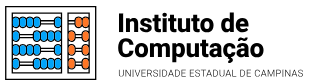
\includegraphics[height=0.9cm]{images/logo_ic.png}
                \hfill
\includegraphics[height=1.2cm]{images/onpce.png}}

\begin{document}
\maketitle

\begin{frame}{Introdução}
    \textbf{\textit{HC Unicamp}}
    \begin{columns}
        \column{0.5\textwidth}
        \begin{itemize}
            \setlength\itemsep{1em}
            \item Hospital de que atende a população de Campinas e região
            \item Atendimento de alta complexidade
            \item Mais de 30 especialidades cirúrgicas eletivas, incluindo de transplantes
        \end{itemize}
        \column{0.5\textwidth}
        \begin{figure}
            \centering
            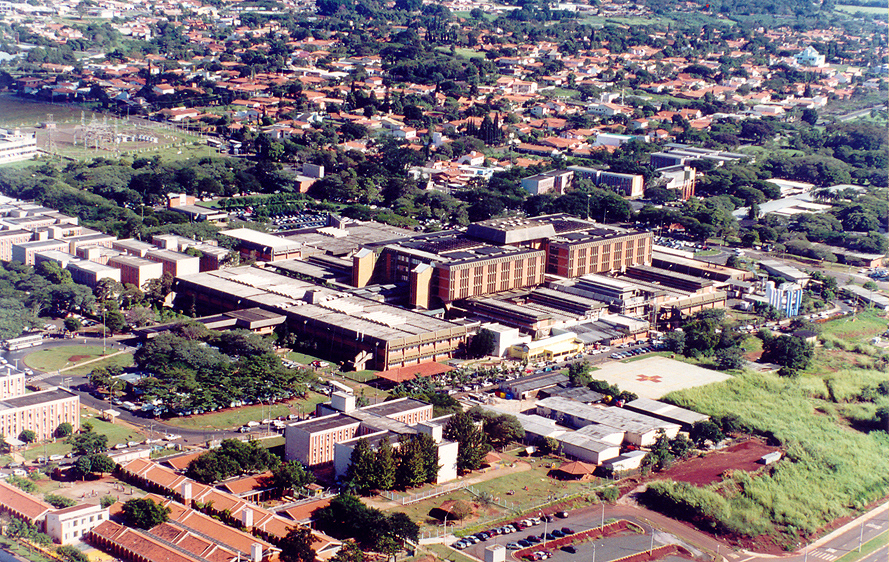
\includegraphics[width=0.8\textwidth]{images/aereahc.jpg}
            \caption{HC Unicamp}
        \end{figure}
    \end{columns}
\end{frame}


\begin{frame}{Introdução}
    \textbf{\textit{Gerenciamento do Centro Cirúrgico}}
    \begin{itemize}
        \setlength\itemsep{1em}
        \item Otimização do uso dos recursos
        \item Redução de custos
        \item Aumento da eficiência
        \item Melhoria na qualidade do atendimento
    \end{itemize}
\end{frame}


\begin{frame}{Planejamento de Salas Cirúrgicas}
    \begin{columns}
        \column{0.5\textwidth}
        A otimização do uso das salas cirúrgicas afeta diretamente:
        \begin{itemize}
            \setlength\itemsep{1em}
            \item Redução do tempo de espera
            \item Redução do tempo de ociosidade
            \item Aumento da eficiência
            \item ``Produção cirúrgica''
        \end{itemize}
        \column{0.5\textwidth}
        \begin{figure}
            \centering
            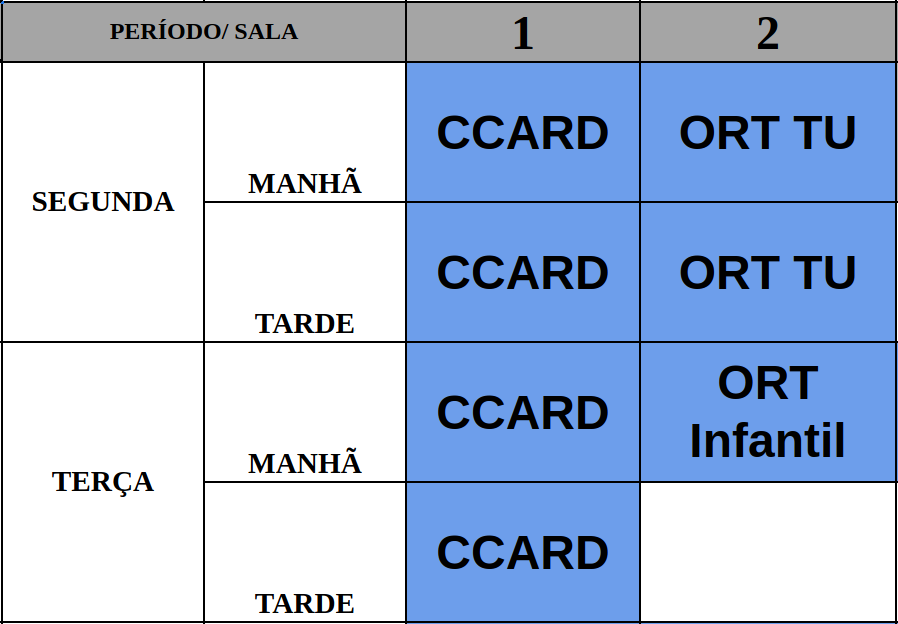
\includegraphics[width=0.8\textwidth]{images/schedule.png}
            \caption{Escala Cirúrgica}
        \end{figure}
    \end{columns}
\end{frame}


\begin{frame}{Restrições Envolvidas}
    Consideramos restriçẽos relacionadas a:
    \begin{itemize}
        % \setlength\itemsep{1em}
        \item Disponibilidade de salas
        \item Disponibilidade de equipes médicas
        \item Demanda mínima de cada especialidade
        \item \alert{Disponibilidade de anestesistas}
        \item \alert{Restrições de transplante}
    \end{itemize}

    Na literatura, outras restrições são consideradas, como:
    \begin{itemize}
        % \setlength\itemsep{1em}
        \item Disponibilidade de equipamentos
        \item Tempo de recuperação
        \item Tempo de limpeza
        \item Tempo de preparação
        \item Tempo de deslocamento
    \end{itemize}
\end{frame}


\begin{frame}{Modelo de Planejamento de Salas Cirúrgicas}
    Cada especialidade precisa ser alocada a pelo menos $\mindeficit$ blocos (demanda mínima)
    \begin{equation}
    \label{eq:m2-2}
        \sum_{\roomidx \in \roomset} \sum_{\blockidx \in \blockset} \blockvar \geq \mindeficit{\specialtyidx} \hspace{2em} \forall\, \specialtyidx \in \specialtyset
    \end{equation}
    
    Para cada especialidade $\specialtyidx \in \specialtyset$, a quantidade de blocos alocados no período de planejamento pode ser, no máximo, $k$ vezes maior do que a demanda $\demand_{\specialtyidx}$, com $k \in [0,1]$
    \begin{equation}
    \label{eq:m2-3}
        \sum_{\roomidx \in \roomset} \sum_{\blockidx \in \blockset} \blockvar \leq (1 + \ub) \cdot \demand_{\specialtyidx} \hspace{2em} \forall\, \specialtyidx \in \specialtyset
    \end{equation}
\end{frame}


\begin{frame}{Modelo de Planejamento de Salas Cirúrgicas}    
    Cada bloco de cada sala deve ser alocado a, no máximo, uma especialidade
    \begin{equation}
    \label{eq:m2-4}
        \sum_{\specialtyidx \in \specialtyset} \blockvar \leq 1 \hspace{2em} \forall\, \roomidx \in \roomset,\, \blockidx \in \blockset
    \end{equation}
    
    Para cada bloco de horário, o número de alocações de especialidades que precisam de anestesista ($\needanest_s = 1$) deve ser igual ou inferior à quantidade de anestesistas disponíveis, já que é exigido um anestesista por alocação de especialidade
    \begin{equation}
    \label{eq:m2-5}
        \sum_{\roomidx \in \roomset} \sum_{\specialtyidx \in \specialtyset} \needanest_{\specialtyidx} \cdot \blockvar \leq \numbersanests_{\blockidx} \hspace{2em} \forall\, \blockidx \in \blockset
    \end{equation}
\end{frame}


\begin{frame}{Modelo de Planejamento de Salas Cirúrgicas}
    Para cada sala, cada bloco de horário, cada especialidade só pode ser alocada em, no máximo, $\specteams$ salas, de acordo com a disponibilidade de times de cirurgia
    \begin{equation}
    \label{eq:m2-6}
        \sum_{\roomidx \in \roomset} \blockvar \leq \specteams_{\blockidx\specialtyidx} \hspace{2em} \forall\, \blockidx \in \blockset,\, \specialtyidx \in \specialtyset
    \end{equation}
    
    Além da restrição da quantidade de times por bloco de horário, temos alguns casos de ter equipe disponível naquele bloco de horário, mas não em todas as salas. Isso acontece porque algumas especialidades tem a liberação para usar algumas salas somente em alguns dias da semana. Então temos a seguinte restrição (fixação de variáveis)
    \begin{equation}
    \label{eq:m2-7}
        \blockvar = 0 \hspace{2em} \forall\, \roomidx \in \roomset,\,\blockidx \in \blockset,\, \specialtyidx \in \specialtyset : \allowedrooms_{\roomidx\blockidx\specialtyidx} = 0
    \end{equation}
\end{frame}
   

\begin{frame}{Modelo de Planejamento de Salas Cirúrgicas}
    Restrição para acoplar as variáveis de alocação $\blockvar$ e as variáveis de blocos sequenciais do mesmo dia $\precvar$, garantindo que, quando $\precvar = 0$, no máximo uma das variáveis de alocação do lado esquerdo será~$1$
    \begin{equation}
    \label{eq:m2-8}
        \blockvar + x_{\roomidx(\blockidx+1)\specialtyidx} - 1 \leq \precvar \hspace{2em} \forall\, \roomidx \in \roomset,\, \blockidx \in \blockset,\,\specialtyidx \in \specialtyset,\, \planninghorizonidx \in \planninghorizonset : \text{ $\blockidx$ e $\blockidx+1$ são blocos do mesmo dia $\planninghorizonidx$}
    \end{equation}
    
    Restrição para acoplar as variáveis de alocação $\blockvar$ e as variáveis de blocos sequenciais do mesmo dia $\precvar$, garantindo que quando $\precvar = 1$, as duas variáveis de alocação serão $1$
    \begin{equation}
    \label{eq:m2-9}
        \blockvar + x_{\roomidx(\blockidx+1)\specialtyidx} \geq 2 \cdot \precvar \hspace{2em} \forall\, \roomidx \in \roomset,\, \blockidx \in \blockset,\,\specialtyidx \in \specialtyset,\, \planninghorizonidx \in \planninghorizonset : \text{ $\blockidx$ e $\blockidx+1$ são blocos do mesmo dia $\planninghorizonidx$}
    \end{equation}
\end{frame}


\begin{frame}{Modelo de Planejamento de Salas Cirúrgicas}
    Restrição de especialidades que precisam de dois blocos (o dia todo) em alguns dias da semana
    \begin{equation}
    \label{eq:m2-10}
        \blockvar = x_{\roomidx(\blockidx+1)\specialtyidx} \hspace{2em} \forall\, \roomidx \in \roomset,\, \blockidx \in \blockmset,\,\specialtyidx \in \specialtymset,\, \planninghorizonidx \in \planninghorizonset : \text{ $\blockidx$ e $\blockidx+1$ são blocos do mesmo dia $\planninghorizonidx$}
    \end{equation}
    
    Restrição que garante que as especialidades de transplante ($\specialtytxset$) tenham uma quantidade par de salas
    \begin{equation}
    \label{eq:m2-11}
        \sum_{\roomidx \in \roomset} \blockvar = 2 \cdot \integervar \hspace{2em} \forall\, \blockidx \in \blockset,\, \specialtyidx \in \specialtytxset
    \end{equation}
\end{frame}


\begin{frame}{Modelo de Planejamento de Salas Cirúrgicas}
    Restrição que garante que as especialidades circunstanciais -- porém prioritárias -- tenham blocos alocados em determinado intervalo de blocos $\blockcset$ , por conta de agendamento (i.e., TMO que precisa de um bloco quando tem agendamento prévio)
    \begin{equation}
    \label{eq:m2-12}
        \sum_{\roomidx \in \roomset} \sum_{\blockidx \in \blockcset} \blockvar = \demand_{\specialtyidx} \hspace{2em} \forall\, \specialtyidx \in \specialtycset
    \end{equation}
    
    Restrição com que todas as proporções de alocação sejam maiores do que uma variável $\balancevar$. Junto da segunda função objetivo, estaremos maximizando a menor proporção de alocação
    \begin{equation}
    \label{eq:m2-13}
         \sum_{\roomidx \in \roomset} \sum_{\blockidx \in \blockset} \frac{\blockvar}{\demand_{\specialtyidx}} \geq \balancevar \hspace{2em} \forall\, \specialtyidx \in \specialtyset
    \end{equation}
\end{frame}


\begin{frame}{Resultados}
    % exemplo de escala antiga feita na mao
    % enfatizar os buracos e a falta de otimizacao
\end{frame}


\begin{frame}{Resultados}
    % exemplo de escala antiga feita na pelo solver, com as mesmas restrições
    % enfatizar que mais blocos foram alocados
\end{frame}


\begin{frame}{Resultados}
    % exemplo de escala antiga feita na pelo solver, com algumsa folgas nas restrições
    % enfatizar que mais blocos foram alocados
\end{frame}

\begin{frame}{Resultados}
    % Gráficos mostrando melhoras ao usar o solver
\end{frame}

\begin{frame}{Conclusões}
    % resumir o que foi feito
    % resumir os resultados
    % possíveis melhorias
\end{frame}

\begin{frame}{Conclusões}
    % dificuldades: linkar com o trabalho do lucas
    % trabalhos futuros
\end{frame}

\end{document}
